\documentclass[12pt,letterpaper]{article}
%\textheight=21cm
%\textwidth=18cm
%\topmargin=2cm
%\oddsidemargin=2.5cm
\usepackage[latin1]{inputenc}
\usepackage{graphicx}

\begin{document}

{\Huge {\rm { \bf Instituto Politecnico Nacional}}}\\
\begin{center}
{\huge {\rm {\em Escuela Superior de C\'omputo}}} \\
\end{center}
\begin{center}
{\Large {\em Tecnolog\'ias para la Web}}\\
\end{center}
\begin{center}
{\Large Alejandro Hern\'andez Hern\'andez}\\
\end{center}
\begin{center}
{\huge {\bf PR\'ACTICA 1}}
\end{center}

\newpage %nueva pagina
{\Huge {\rm {\bf Introducc\'ion}}}
\\
\begin{flushleft}
HTML {\em HyperText Markup Languaje} es un lenguaje que nos permite dise\~nar una pagina web en su forma mas simple o b\'asica.
\\Se denomina {\em Hypertext} o {\em Hipertexto} porque se conecta una pagina web con otra, y usa {\em Markup} o {\em marcado} para anotar textos y contenido que se muestran en el navegador.
\\
HTML actualmente incorpora otras tecnologias para su funcionamiento, como son estilos para personalizacion de paginas web ({\bf CSS}) o para describir su funcionalidad ({\bf JavaScript}).\\
\vspace{1.5cm}
{\large {\em Apache}}
\\
{\em Apache} es un servidor web que implementa el protocolo {\bf HTTP/1.1}, y permite emular un sitio virtual. Este servidor se encuentra a la espera de una solicitud de algun navegador que se encuentre en el host, y hace una respuesta a dicha peticion, transfiriendo codigo HTML como datos en red.
\\
\vspace{1.5cm}
La finalidad es comprender el funcionamiento del servidor {\em Apache} y el uso de {\em HTML}, y el comienzo de la utilizacion de ambos en conjunto.


\end{flushleft}

\newpage
{\Huge {\rm {\bf Desarrollo}}}
\begin{flushleft}
Lo primero que se realiza, es instalar {\em {\bf Apache2}} en cualquier distribuci\'on {\em Linux}. Para ello, abrimos una terminal y ejecutaremos el comando \\

\begin{center}
\fboxsep 12pt
\begin{minipage}[t]{6cm}
{\bf sudo apt-get install apache2}
\end{minipage}
\end{center}
(ver Figure 1)
%aqui hay que poner una imagen xd

%aquiva otra imagen


Una vez instalado, nos aseguramos de que nuestro servidor este {\rm {\em "arriba"}} o {\rm {\em encendido}}, ejecutamos: 
\begin{center}
\fboxsep 12pt
\begin{minipage}[t]{3cm}
{\bf sudo su}
\end{minipage}
\end{center}

Nos pedir\'a la contrase\~na, y una vez en modo superusuario, ejecutamos: 
\begin{center}
\fboxsep 12pt
\begin{minipage}[t]{6cm}
{\bf /etc/init.d/apache2 status}
\end{minipage}
\end{center}

Aqu\'i tenemos 2 opciones:\\si est\'a encendido, aparece (ver Figure 2)%\\aqui va otra imagen\\

Si est\'a apagado, aparece (ver Figure 3)% \\aqui va otra imagen xd\\
\\
En caso de que est\'e apagado, ejecutaremos el siguiente comando, en modo superusuario: 
\begin{center}
\fboxsep 12pt
\begin{minipage}[t]{6cm}
{\bf /etc/init.d/apache2 restart}
\end{minipage}
\end{center}
Y al ejecutar
\begin{center}
\fboxsep 12pt
\begin{minipage}[t]{6cm}
{\bf /etc/init.d/apache2 status}
\end{minipage}
\end{center}
debe de aparecer (ver Figure 4)% \\aqui va otra imagen xd\\

\vspace{3cm}
Una vez seguros de que el servidor esta encendido, en un editor de texto, llamese {\em {\bf Sublime text, Gedit o editor de texto, Leafpad}}, procedemos a escribir nuestro primer codigo {\bf HTML} o nuestra {\em primera p\'agina web} (ver Figure 5)%:\\aqui va otra imagen xd
\begin{center}
\fboxsep 12pt
{\bf CODIGO: \\}
\begin{verbatim}
<html>
<body>
Hola mundo
</body>
</html>
\end{verbatim}
\end{center}
\end{flushleft}
 %hasta aqui llegue xdxdxdxd
%aqui otra imagen xd

Luego, la guardamos en el directorio
\begin{center}

\begin{minipage}[t]{6cm}
\fboxsep 12pt
{\bf /var/www/html/nombre\_pagina.html}
\end{minipage}
\end{center}
En el caso personal, se llam\'o {\bf {\em pract1.html}}\\
Una vez hecho lo anterior, abrimos el explorador (en mi caso, fu\'e {\bf {\em Mozilla Firefox}}), y en la barra de direcciones escribimos: 
\begin{center}
\begin{minipage}[t]{6cm}
\fboxsep 12pt
{\bf localhost/nombre\_pagina.html}
\end{minipage}
\end{center}
que, en mi caso, fu\'e {\bf {\em localhost/pract1.html}} (ver Figure 6) y se muestra el contenido con el {\em estilo} de HTML.
\newpage
%aqui van las imagenes
\begin{center}
\begin{figure}[h]
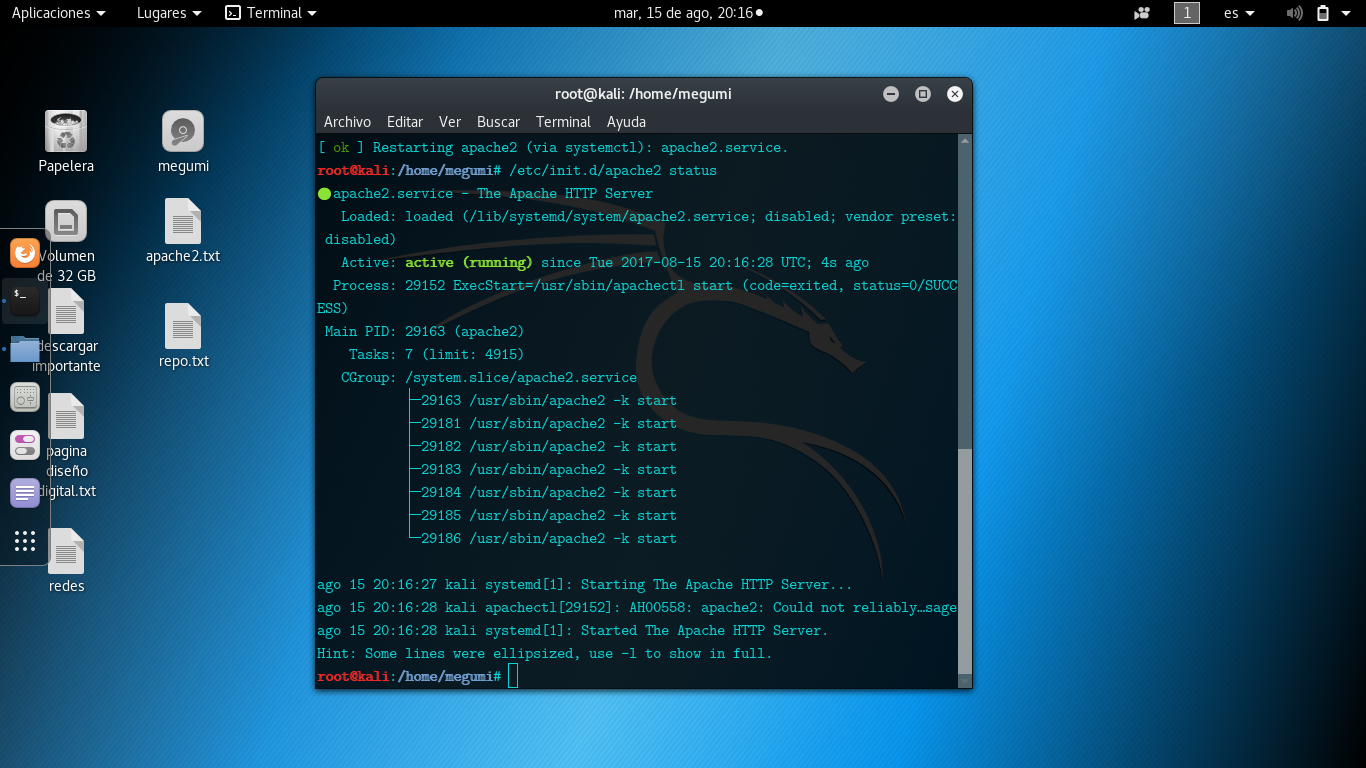
\includegraphics[width=400pt]{./imgs/2.png}
\caption{figura 1}\label{figure 1}
\end{figure}

%figura 2
\begin{figure}[h]
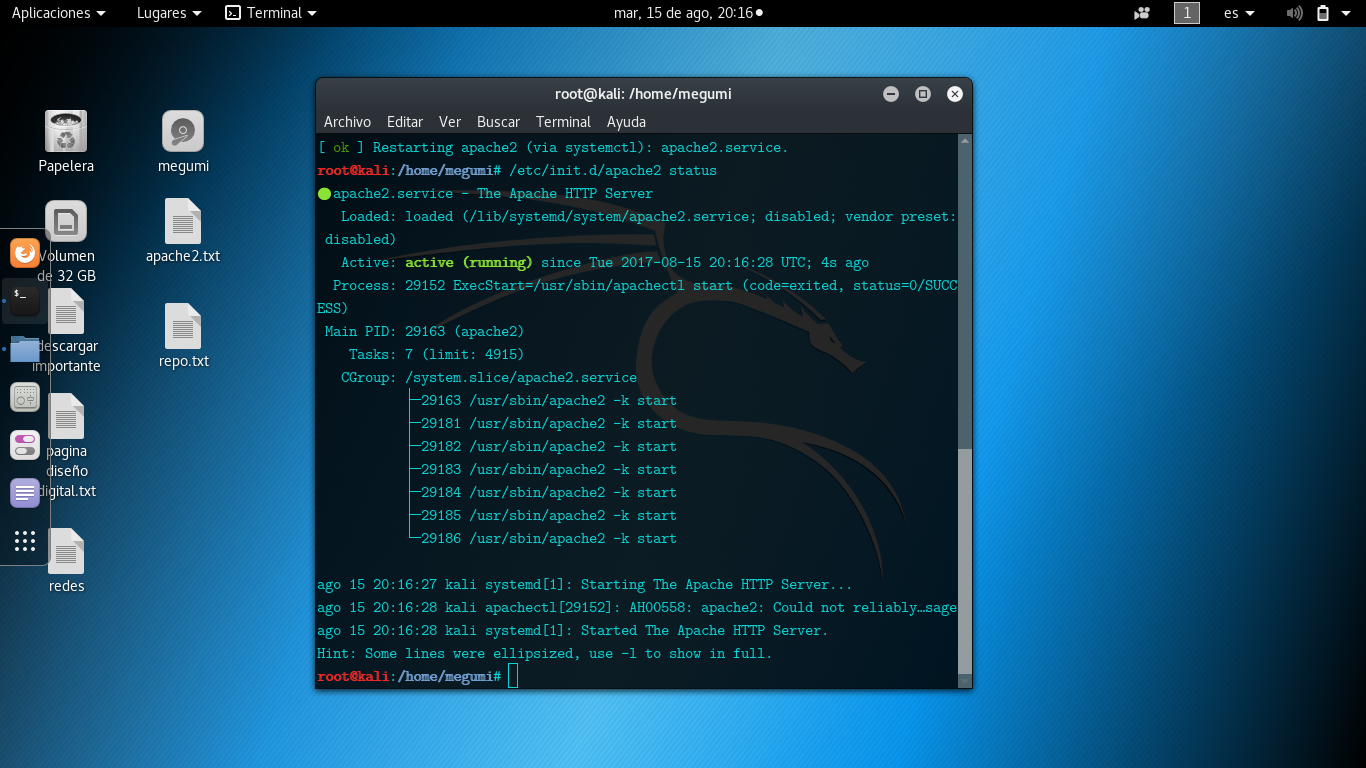
\includegraphics[width=400pt]{./imgs/2.png}
\caption{figura 2}\label{figure 2}
\end{figure}

%figura 3
\begin{figure}[!ht]
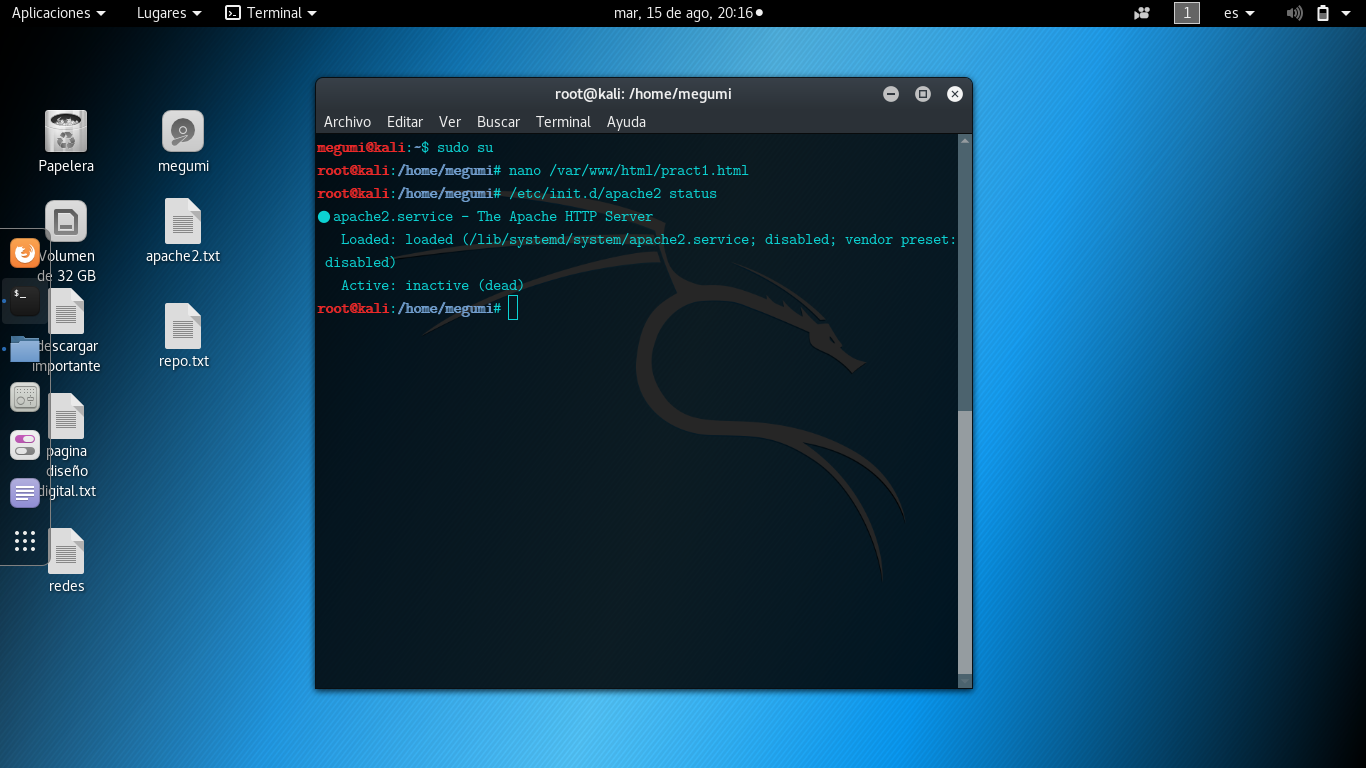
\includegraphics[width=400pt]{./imgs/1.png}
\caption{figura 3}\label{figure 3}
\end{figure}

%figura 4
\begin{figure}[!ht]
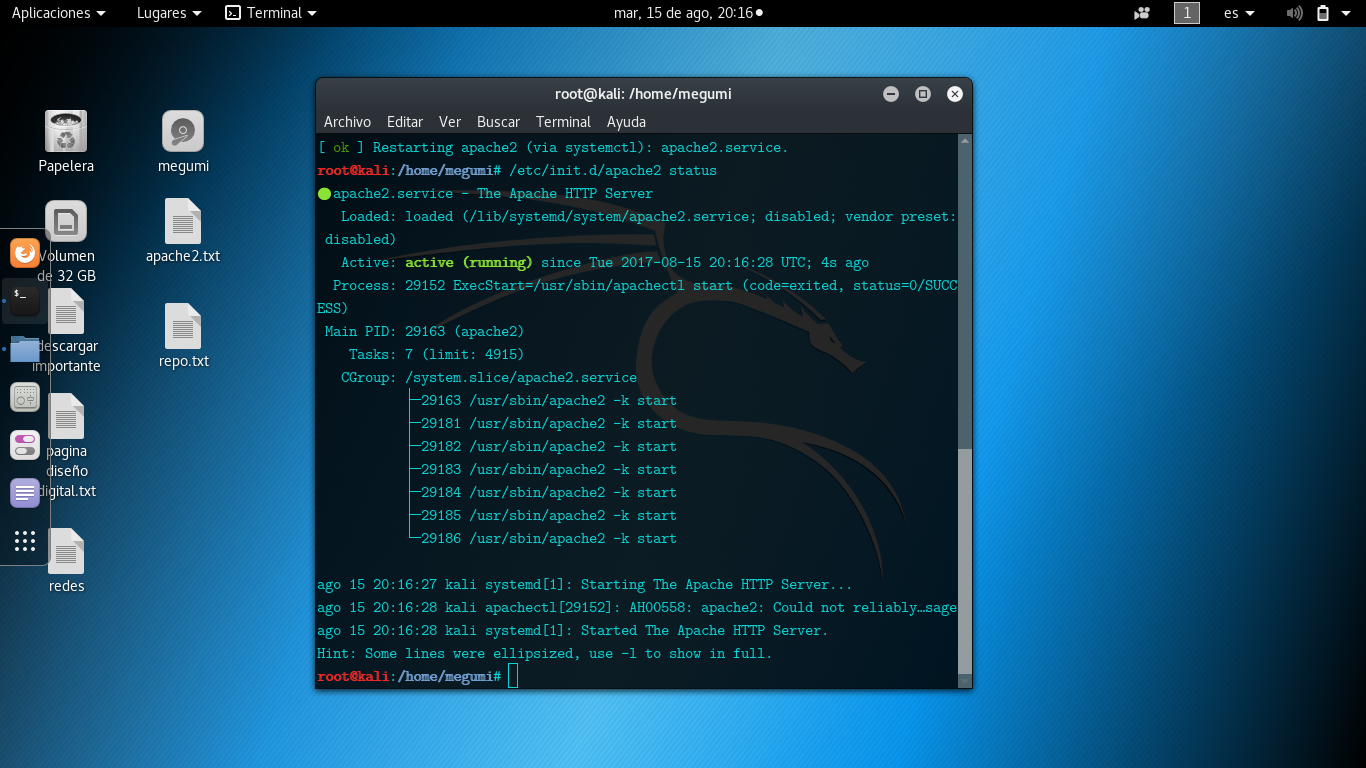
\includegraphics[width=400pt]{./imgs/2.png}
\caption{figura 4}\label{figure 4}
\end{figure}

%figura 5
\begin{figure}[!ht]
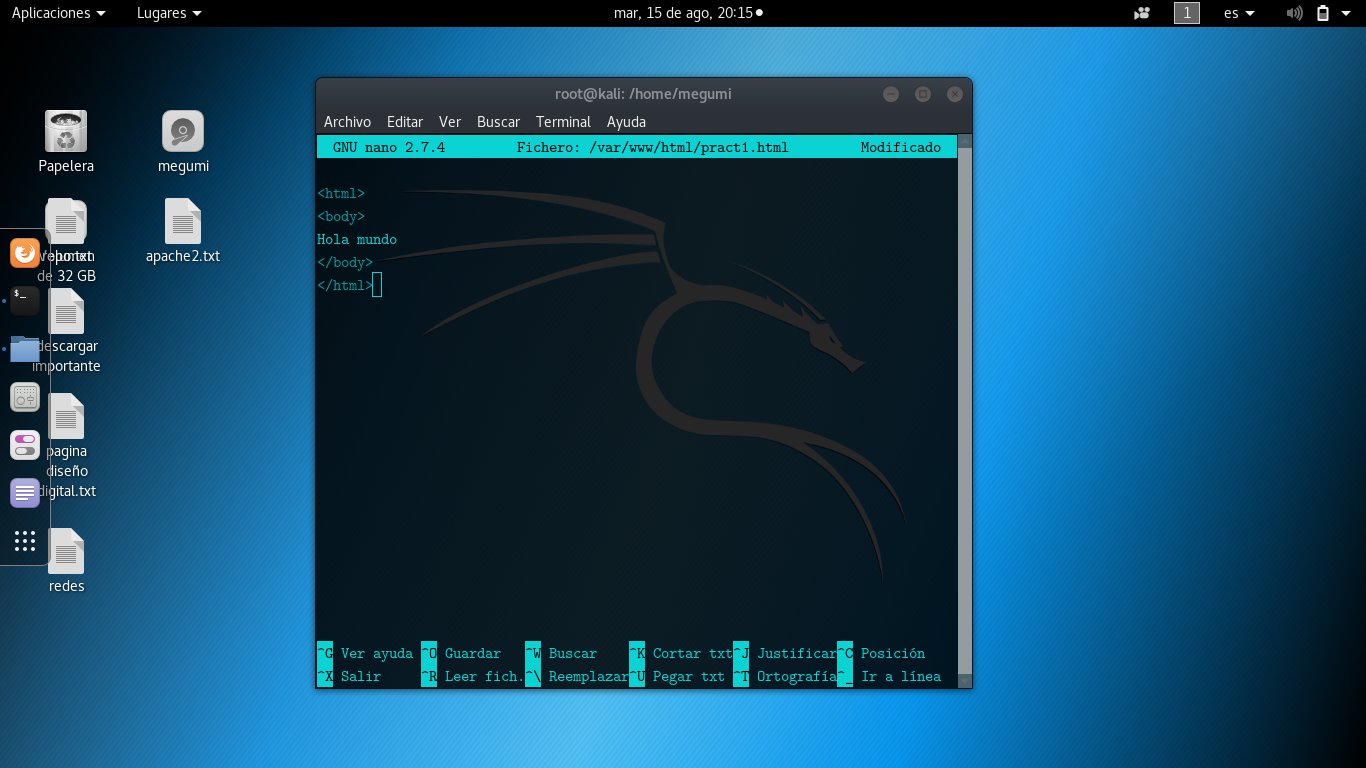
\includegraphics[width=400pt]{./imgs/3.png}
\caption{figura 5}\label{figure 5}
\end{figure}

%figura 6
\begin{figure}[h]
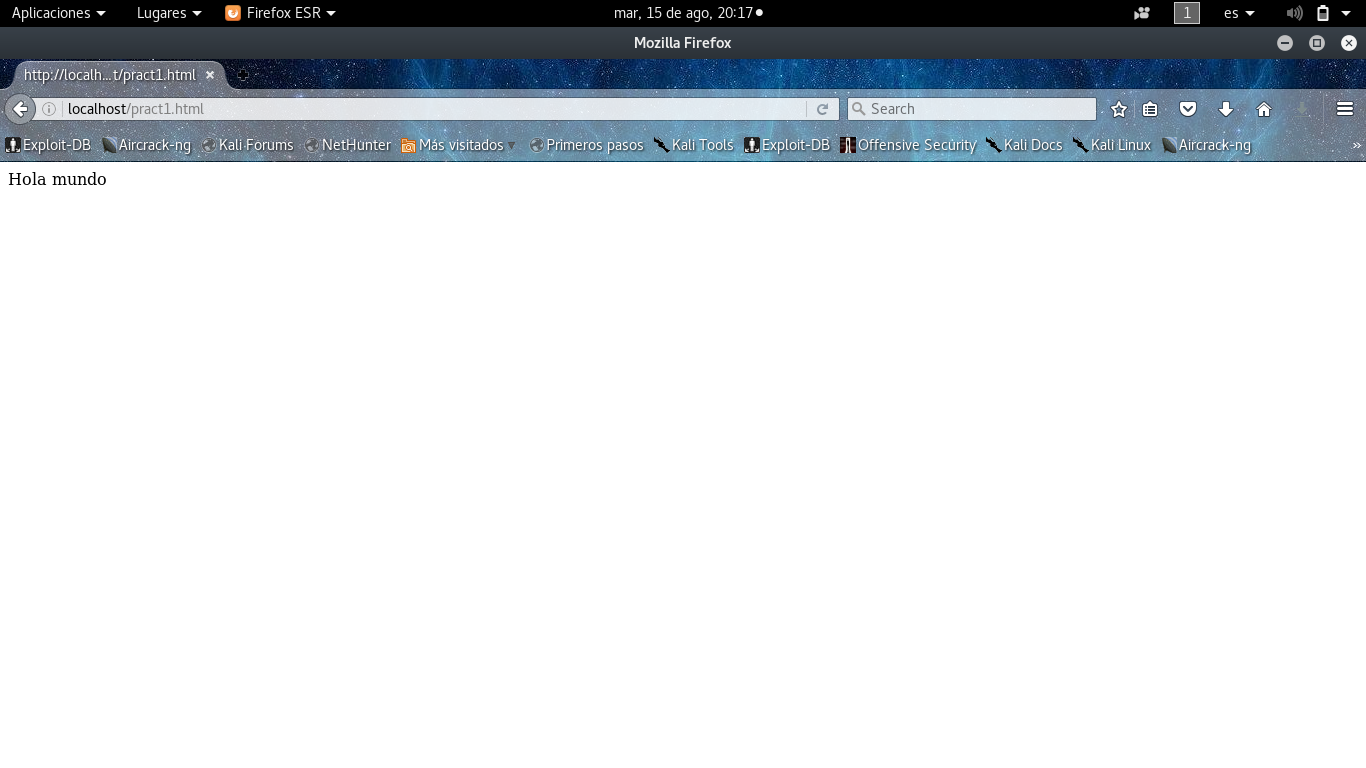
\includegraphics[width=400pt]{./imgs/6.png}
\caption{figura 6}\label{figure 6}
\end{figure}
\end{center}



\end{document}
